\chapter{混合、振荡、电偶极矩与场算符}

我们从一个稍微偏离所宣称主题的问题开始，这个问题关于中微子。有证据表明中微子具有质量，并且中微子类型会混合。如果质量并不全都相同，那么一种类型如何能在不违反能量守恒的情况下转变为另一种类型？

这个问题指向一个贯穿整个量子力学的模式：系统被制备或探测时所处的态，不必是使其哈密顿量对角化的态。具有确定能量的态只会获得一个相位。一个由若干能量叠加而成的制备态会发生变化，因为它的各分量获得不同的相位。这一区分将把我们从一个双势阱带到中微子振荡和自旋进动。在插入一段关于电子电偶极矩的内容之后，我们将回到二次量子化，并在算符层面看到同样的位置--动量傅里叶结构。

\section{混合才是真正的问题}

中微子不必全都具有相同的质量。能量本征态彼此之间不会混合；每一个都独立演化。我们所称的中微子的\emph{类型}，或味，是与它如何产生和探测相关联的，而一个味态可以是质量-能量本征态的线性组合。示意地，
\begin{equation}
|\text{type}\rangle = \sum_n c_n |E_n\rangle .
\end{equation}
因此正确的陈述并不是能量本征态彼此转变，而是被称为``电子中微子''或``{\proseunicodefont μ}子中微子''的态本身不必是能量本征态。

\begin{classroomqa}
\lecturetimestamp{00:00:09}
\audiencequestion{如果中微子具有不同质量，它们如何能在能量保持守恒的同时混合？}
\lecturerresponse{质量-能量本征态不会彼此转变。电子味、{\proseunicodefont μ}子味和{\proseunicodefont τ}味态是这些本征态的不同线性组合。每个质量分量以自己的相位演化，而干涉改变味概率，同时不违反能量守恒。}
\end{classroomqa}

这种结构有许多例子。最明显的一个从对称双势阱中的粒子开始。

\section{对称双势阱与近似定域态}

考虑一个在对称双势阱势中运动的粒子，两个极小值之间有一个高势垒。如果把势垒取为无限高，那么左势阱和右势阱将完全解耦。人们可以像右势阱不存在那样求解左势阱，反之亦然。近似基态波函数于是将是一个左定域态\(\psi_L\)和一个右定域态\(\psi_R\)，二者具有相同的能量\(E\)。

在每个孤立势阱中，基态具有熟悉的定性性质：它是光滑的，没有节点，并且处于与束缚条件相容的最低可能能量。把高的中心势垒想象成一堵砖墙。把它当作无限高只是一种近似，但它给了我们一对有用的定域态作为出发点。

\begin{figure}
\centering
\begin{adjustbox}{max width=\linewidth}
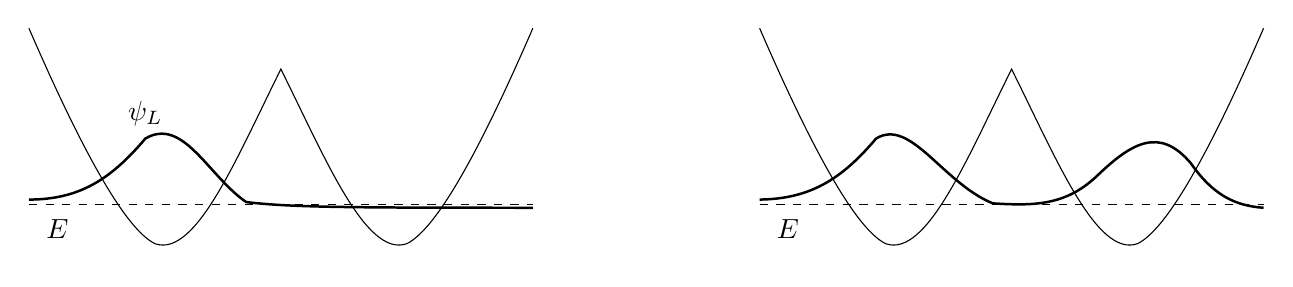
\begin{tikzpicture}[x=0.8cm,y=0.8cm]
\begin{scope}[shift={(-5.8,0)}]
\draw (-4,2.7) .. controls (-3.35,1.2) and (-2.55,-0.45) .. (-2.0,-0.72)
      .. controls (-1.35,-0.95) and (-0.7,0.65) .. (0,2.05)
      .. controls (0.7,0.65) and (1.35,-0.95) .. (2.0,-0.72)
      .. controls (2.55,-0.45) and (3.35,1.2) .. (4,2.7);
\draw[dashed] (-4,-0.10) -- (4,-0.10);
\node at (-3.55,-0.48) {$E$};
\draw[line width=0.9pt] (-4,-0.02) .. controls (-3.2,-0.02) and (-2.7,0.30) .. (-2.15,0.95)
      .. controls (-1.55,1.30) and (-1.15,0.35) .. (-0.55,-0.06)
      .. controls (0.15,-0.14) and (0.9,-0.15) .. (4,-0.15);
\node at (-2.15,1.35) {$\psi_L$};
\end{scope}
\begin{scope}[shift={(5.8,0)}]
\draw (-4,2.7) .. controls (-3.35,1.2) and (-2.55,-0.45) .. (-2.0,-0.72)
      .. controls (-1.35,-0.95) and (-0.7,0.65) .. (0,2.05)
      .. controls (0.7,0.65) and (1.35,-0.95) .. (2.0,-0.72)
      .. controls (2.55,-0.45) and (3.35,1.2) .. (4,2.7);
\draw[dashed] (-4,-0.10) -- (4,-0.10);
\node at (-3.55,-0.48) {$E$};
\draw[line width=0.9pt] (-4,-0.02) .. controls (-3.2,-0.01) and (-2.7,0.30) .. (-2.15,0.95)
      .. controls (-1.6,1.28) and (-1.1,0.25) .. (-0.30,-0.08)
      .. controls (0.35,-0.12) and (0.85,-0.12) .. (1.35,0.35)
      .. controls (1.9,0.88) and (2.35,1.15) .. (2.85,0.55)
      .. controls (3.2,0.05) and (3.55,-0.12) .. (4,-0.15);
\end{scope}
\end{tikzpicture}
\end{adjustbox}
\caption{开场板书的清晰重绘。左边是单侧试探态\(\psi_L\)，它是通过假装势垒实际上无限高而得到的。右边是同一个波函数对称地穿过势垒延拓后的情形，用以说明最终产生真正偶宇称基态的那种微小但非零的泄漏。}
\end{figure}

然而，在量子力学中，势垒并非真正无限高。势垒区域中的波函数并不严格为零；它只是非常小。这种微小的泄漏就是全部关键所在。正是它把左右近似转化为一个真正的混合问题。

\section{宇称本征态与指数能级分裂}

现在，定域图像被一个定理打断：如果势是对称的，那么精确的能量本征函数可以被选为在反射下要么对称、要么反对称。

\begin{theorem}
如果在一维中\(V(x)=V(-x)\)，那么哈密顿量的本征函数可以被选为满足
\[
\psi(x)=\psi(-x)
\qquad \text{or} \qquad
\psi(x)=-\psi(-x).
\]
\end{theorem}

现在来了修正。单侧态\(\psi_L\)和\(\psi_R\)既不是对称的，也不是反对称的，因此它们不可能是完整哈密顿量的精确本征态。只有当势垒很高时，它们才是良好的近似态。真正的本征态是对称组合和反对称组合，
\begin{align}
\psi_+ &= \frac{\psi_L+\psi_R}{\sqrt{2}},\\
\psi_- &= \frac{\psi_L-\psi_R}{\sqrt{2}}.
\end{align}
使用将留在黑板上的记号，把它们的能量记为
\begin{align}
H\psi_+ &= (E_1-\epsilon)\psi_+,\\
H\psi_- &= (E_1+\epsilon)\psi_-.
\end{align}
因此总分裂为
\begin{equation}
\Delta E = (E_1+\epsilon)-(E_1-\epsilon)=2\epsilon .
\end{equation}

\begin{figure}[htbp]
\centering
\includegraphics[width=0.92\linewidth]{lecture_08_frame_02.png}
\caption{双势阱中对称延拓的波函数。其振幅在势垒下方很小但非零，这正是能级分裂的起源。}
\lectureframe{00:06:19}
\end{figure}

\begin{figure}
\centering
\begin{tikzpicture}[x=1cm,y=1cm]
\draw[->] (0,0) -- (0,3);
\node[left] at (0,2.8) {energy};
\draw (-0.35,1.60) -- (0.35,1.60);
\node[left] at (-0.45,1.60) {$\psi_L,\psi_R$};
\node at (1.7,1.60) {$\Longrightarrow$};
\draw (3.0,1.32) -- (3.75,1.32);
\draw (3.0,1.88) -- (3.75,1.88);
\draw[dashed] (2.8,1.60) -- (3.95,1.60);
\node[right] at (3.9,1.32) {$\psi_+,\ E_1-\epsilon$};
\node[right] at (3.9,1.88) {$\psi_-,\ E_1+\epsilon$};
\node[below] at (3.37,1.60) {$E_1$};
\end{tikzpicture}
\caption{隧穿分裂的板书逻辑。近似的左态和右态几乎简并，但精确的对称和反对称本征态被一个很小的量\(2\epsilon\)分裂。}
\end{figure}

能级的排序承载着物理要点。对称态的能量略低，因为它在势垒区域更平滑；允许波函数泄漏并对称地延续会使能量降低一个极小的量。反对称态的能量略高，因为一维中的第一激发态有一个节点，而在这个对称问题中该节点位于中点。额外的曲率需要消耗动能。

这一效应非常小，在势垒宽度和高度上呈指数级小。这里我们不需要显式的WKB公式；重要的是分裂是真实的但极其微小。还要记住，波函数的整体符号不携带任何物理信息。将\(\psi_-\)替换为\(-\psi_-\)不会改变状态。

\section{时间演化与左右振荡}

现在问一个动力学问题：如果我们将粒子放在左侧势阱中会发生什么？这是决定性的一步，因为振荡正是同一混合现象在时间依赖上的表现。

逆关系为
\begin{align}
\psi_L &= \frac{\psi_+ + \psi_-}{\sqrt{2}},\\
\psi_R &= \frac{\psi_+ - \psi_-}{\sqrt{2}}.
\end{align}
因此初始局域在左侧的态为
\begin{equation}
\psi(0)=\psi_L=\frac{\psi_+ + \psi_-}{\sqrt{2}}.
\end{equation}
它不是能量本征态，因此必然发生非平凡演化。

我们采用标准的Schr\"odinger约定\(e^{-iEt}\)。整体相位没有可观测效应；只有两个能量分量之间的相对相位才能将概率从一个势阱转移到另一个势阱。

在该约定下，
\begin{equation}
\psi(t)=\frac{1}{\sqrt{2}}\left(e^{-i(E_1-\epsilon)t}\psi_+ + e^{-i(E_1+\epsilon)t}\psi_-\right).
\end{equation}
这是板书公式整理后的版本。现在提取公共相位：
\begin{equation}
\psi(t)=\frac{e^{-iE_1 t}}{\sqrt{2}}\left(e^{i\epsilon t}\psi_+ + e^{-i\epsilon t}\psi_-\right).
\end{equation}
现在一个相位沿单位圆朝一个方向旋转，另一个则朝相反方向旋转。状态之所以变化，仅仅是因为这两个相位逐渐失步。

为了明确看到左右振荡，代入\(\psi_\pm\)的定义：
\begin{align}
\psi(t)
&= \frac{e^{-iE_1 t}}{2}
\left[e^{i\epsilon t}(\psi_L+\psi_R)+e^{-i\epsilon t}(\psi_L-\psi_R)\right] \\
&= \frac{e^{-iE_1 t}}{2}
\left[(e^{i\epsilon t}+e^{-i\epsilon t})\psi_L+(e^{i\epsilon t}-e^{-i\epsilon t})\psi_R\right] \\
&= e^{-iE_1 t}\left[\psi_L\cos(\epsilon t)+i\,\psi_R\sin(\epsilon t)\right].
\end{align}
这是本章关键的完整推导。在双态近似下，当\(\psi_L\)和\(\psi_R\)正交归一时，概率为
\begin{equation}
P_L(t)=\cos^2(\epsilon t),
\qquad
P_R(t)=\sin^2(\epsilon t).
\end{equation}
因此系统发生振荡。在中间时刻它确实处于叠加态；例如，当\(\epsilon t=\pi/4\)时，两侧的概率相等。相位连续演化，局域化也随之连续变化。

黑板推导确定了相对符号首次翻转的时刻。人们问何时
\begin{equation}
e^{-i\epsilon t}=-\,e^{i\epsilon t},
\end{equation}
这是黑板上可见的里程碑。两边相乘得到
\begin{equation}
e^{2i\epsilon t}=-1.
\end{equation}
对于首次出现，
\begin{equation}
2\epsilon t=\pi,
\qquad\text{so}\qquad
t_{L\to R}=\frac{\pi}{2\epsilon}.
\end{equation}

\begin{figure}[htbp]
\centering
\includegraphics[width=0.94\linewidth]{lecture_08_frame_05.png}
\caption{黑板上的相对相位计算。当\(e^{2i\epsilon t}=-1\)时，两个能量分量变为相反，给出第一个转移时间\(2\epsilon t=\pi\)。排版推导使用一个一致的Schr\"odinger相位约定。}
\lectureframe{00:17:52}
\end{figure}
在该时刻，
\begin{equation}
\psi(t_{L\to R}) \propto \frac{\psi_+-\psi_-}{\sqrt{2}}=\psi_R.
\end{equation}
整体相位无关紧要。重要的是，最初置于左侧的粒子已演化为右局域态。再经过一个相等的时间间隔后，它又摆回原处。混合与振荡相伴而生。

方程是明确的：小的\(\epsilon\)意味着缓慢的振荡和较长的转移时间。两个局域态都没有确定的能量，但两个精确的能量分量守恒能量，并完全按照应有的方式演化。

\section{中微子、氨与自旋类比}

双势阱为我们提供了最初中微子问题的模板。与电子一起产生的中微子称为电子中微子；与{\proseunicodefont μ}子一起产生的称为{\proseunicodefont μ}中微子。这些味标签描述的是产生和探测通道。具有确定质量、因而在固定动量下具有确定自由粒子能量的态构成另一个基。

在最简单的双态、最大混合的漫画式描述中，
\begin{equation}
|\nu_e\rangle \sim \frac{|m_1\rangle+|m_2\rangle}{\sqrt{2}},
\qquad
|\nu_\mu\rangle \sim \frac{|m_1\rangle-|m_2\rangle}{\sqrt{2}},
\end{equation}
其中质量本征态扮演\(\psi_+\)和\(\psi_-\)的角色，味态扮演\(\psi_L\)和\(\psi_R\)的角色。真实的中微子混合使用非平凡的混合矩阵，而不是这些相等的系数，但其机制在这里已经可见。

电子中微子是在涉及电子的过程中产生的，正如一个粒子可以被放入左势阱中一样。在短距离飞行中，它的两个质量成分积累的相位几乎相同，因此相互作用仍然将其识别为电子味。在长基线中，它们的相位分离。之后的带电流相互作用则可能产生{\proseunicodefont μ}子而不是电子：该态已经获得了{\proseunicodefont μ}子味成分。在不同距离或能量下重复实验，就会揭示出振荡。

这与能量守恒没有冲突。质量-能量本征态所做的正是本征态应该做的事情。演化的是味叠加态。在相对论极限下，可观测的相对相位由质量平方差决定，示意性地为
\begin{equation}
\Delta\phi_{ij}\simeq \frac{\Delta m_{ij}^{,2}L}{2E}.
\end{equation}
因此，振荡表明并非所有中微子质量都可以相同；至少有两个质量本征态的质量不同。

\begin{classroomqa}
\lecturetimestamp{00:24:06}
\audiencequestion{在双势阱例子中，是什么决定了小分裂\(\epsilon\)？}
\lecturerresponse{它取决于粒子质量以及势垒的高度和宽度。隧穿对这些细节呈指数敏感，因此势垒的适度变化可以导致\(\epsilon\)产生很大的相对变化。}
\end{classroomqa}

\begin{classroomqa}
\lecturetimestamp{00:24:26}
\audiencequestion{这种振荡现象实际上已经被观测到了吗？}
\lecturerresponse{是的。隧穿分裂在普通量子系统中被观测到，而味振荡在中微子中被观测到。其微观机制不同，但两者都实现了相同的两态相位演化。}
\end{classroomqa}

\begin{classroomqa}
\lecturetimestamp{00:24:34}
\audiencequestion{中微子振荡如何与中微子质量相联系？}
\lecturerresponse{传播的本征态具有不同的质量，因此积累不同的相位。它们的干涉改变了味组成。在现实的相对论处理中，控制振荡的是质量平方差，而不是单个粒子字面意义上随时间变化的质量。}
\end{classroomqa}

\begin{classroomqa}
\lecturetimestamp{00:25:02}
\audiencequestion{中微子质量仅仅是流行理论，还是实验事实？}
\lecturerresponse{振荡是实验事实，并且它要求非零的质量差。绝对质量标度是一个单独的、更困难的测量问题，但每个中微子都无质量的最小图像已被实验排除。}
\end{classroomqa}

\subsection{氨反转：一个字面意义上的势垒}

氨分子\(\mathrm{NH}_3\)呈三角锥形：三个氢原子构成一个平面，氮原子位于该平面的一侧。存在一种氮原子位于另一侧的等价构型。这两种局域化构型并不是精确的定态。氮原子可以隧穿通过氢平面，产生对称和反对称能量本征态以及一个小的反转分裂。这就是氨微波激射器中相同数学的物理起源。

\begin{classroomqa}
\lecturetimestamp{00:25:11}
\audiencequestion{在氨中，势垒是氮原子穿过氢平面的那种构型吗？}
\lecturerresponse{是的。分子能量在两种锥形构型中都取极小值，而平面构型则更高。隧穿通过该构型将两侧耦合起来。}
\end{classroomqa}

\begin{classroomqa}
\lecturetimestamp{00:27:10}
\audiencequestion{电子中微子和{\proseunicodefont μ}中微子之间对应的物理势垒是什么？}
\lecturerresponse{不存在字面意义上的空间势垒。这个类比是代数性的：中微子哈密顿量中的非对角耦合混合了味基。在氨中，该耦合来自隧穿；对于中微子，它是质量和混合结构的一部分。}
\end{classroomqa}

\subsection{自旋进动：没有隧穿的混合}

我们在自旋中已经遇到过同样的代数。取两个态\(|\uparrow_z\rangle\)和\(|\downarrow_z\rangle\)。没有磁场时它们是简并的。现在打开沿\(x\)方向的磁场。能量本征态不再是\(z\)本征态，而是\(x\)偏振态。使用黑板上临时的左--右名称，
\begin{align}
|L_x\rangle &= \frac{|\uparrow_z\rangle+|\downarrow_z\rangle}{\sqrt{2}},\\
|R_x\rangle &= \frac{|\uparrow_z\rangle-|\downarrow_z\rangle}{\sqrt{2}}.
\end{align}
这些正是\(\psi_+\)和\(\psi_-\)的直接类比。与磁场同向和反向排列的磁矩具有略微不同的能量。如果这些能量是\(E\mp\epsilon\)，那么一个初始向上的自旋演化为
\begin{equation}
|\uparrow_z,t\rangle
= e^{-iEt}\left[\cos(\epsilon t)\,|\uparrow_z\rangle
+ i\sin(\epsilon t)\,|\downarrow_z\rangle\right].
\end{equation}
这与双势阱的公式相同，只是现在连续演化是绕\(x\)轴的自旋进动。从\(+z\)出发，自旋经过横向方向，在半个进动周期后到达\(-z\)，再经过半个周期后返回。对\(S_z\)的测量仍然只给出向上或向下；连续变化的自旋态决定它们的概率。该机制不需要隧穿。它只要求哈密顿量在一个不同于制备基的基中是对角的。

\begin{classroomqa}
\lecturetimestamp{00:32:25}
\audiencequestion{在这个图像中，{\proseunicodefont τ}中微子会发生什么？}
\lecturerresponse{它也会混合。真实问题有三个味态和三个质量态，因此一个三乘三混合矩阵取代了二态旋转。相位干涉原理不变。}
\end{classroomqa}

\begin{classroomqa}
\lecturetimestamp{00:32:57}
\audiencequestion{在横向磁场施加后立即，自旋仍然向上吗，它能指向我们或背离我们吗？}
\lecturerresponse{在极短的时间内它仍然几乎肯定是向上的，带有很小的向下概率。该态绕磁场轴连续进动，并经过横向的\(\pm y\)方向，而如果它开始时垂直于\(x\)方向的磁场，则保持垂直。沿任意选定轴的测量仍然给出该轴的一个离散本征值。}
\end{classroomqa}

\begin{classroomqa}
\lecturetimestamp{00:34:30}
\audiencequestion{磁场被选得弱，是为了让自旋从不指向磁场方向吗？}
\lecturerresponse{不是。几何来自绕磁场轴的进动，而不是来自磁场的弱。弱磁场只是使能级分裂和进动频率变小，给出类似于中微子例子的缓慢振荡。}
\end{classroomqa}

中微子混合的强度和微小的中微子质量是一些参数，其更深层的起源并未由最初表述的最小标准模型解释。因此中微子质量指向超出该最小模型，尽管观测到的尺度非常小，并且可能反映遥远能量尺度上的物理。

\begin{classroomqa}
\lecturetimestamp{00:36:27}
\audiencequestion{振荡是我们知道中微子有质量的原因吗？}
\lecturerresponse{它是传播分量具有不同质量的决定性直接证据。如果所有相关分量都严格无质量且简并，它们就不会积累任何依赖质量的相对相位，也就不会有这种真空味振荡。}
\end{classroomqa}

\begin{classroomqa}
\lecturetimestamp{00:37:57}
\audiencequestion{在半个周期时，中微子应该一半像电子味、一半像{\proseunicodefont μ}子味吗？}
\lecturerresponse{在理想对称的二态模型中，相等概率出现在完整概率周期的四分之一处，而完全转化出现在第一个极大值处。真实的三味振荡具有不相等的混合角、多个频率、自旋螺旋度约束和物质效应，因此完全对称转化并非普遍情形。}
\end{classroomqa}

\begin{classroomqa}
\lecturetimestamp{00:38:36}
\audiencequestion{如果质量分量不同，太阳中微子的速度必须改变以守恒动量吗？}
\lecturerresponse{一个味态是具有固定质量的分量的相干叠加；它的质量不是随时间振荡的经典量。在常见的等动量描述中，各分量具有略微不同的能量和群速度，而在等能量描述中，它们具有略微不同的动量。当一致处理时，两种约定给出相同的可观测振荡相位。}
\end{classroomqa}

这种相位演化解决了旧的太阳中微子短缺问题。早期探测器主要对电子中微子敏感，因此以电子味离开太阳的中微子可能部分以{\proseunicodefont μ}子味或{\proseunicodefont τ}味到达并逃逸该通道。详细的太阳计算包括三味混合和物质效应，但概念上的教训已经存在于双势阱中：制备和传播使用不同的基。

\section{插曲：电偶极矩、对称性与``电子是球''的说法}

既然我们已经在谈论粒子唯象学，不妨暂时离开形式化的数学。一篇科普文章在描述一个新的电子电偶极矩上限时说，电子已被证明是一个球。这个口号混淆了三个不同的问题：电偶极矩测量的是什么，旋转对称性对量子态意味着什么，以及实验实际约束了什么。

\subsection{测量了什么？}

被测量、或者更确切地说是被给出上限的，是电子的电偶极矩。对于分离的电荷\(\pm q\)，偶极矩为
\begin{equation}
\mathbf d = q\,\boldsymbol{\ell},
\end{equation}
其中\(\boldsymbol{\ell}\)是分离矢量。非零的偶极矩意味着电荷分布相对于某个中心发生了位移。

然而对于电子，相关的问题并不仅仅是电荷是否沿某个任意方向偏离中心。电子有自旋，因而有一个轴。它也有磁矩。物理上有意义的问题是，电荷的位移与那个轴之间是否存在关联：
\begin{equation}
\mathbf d_e \parallel \boldsymbol{\mu}_e
\qquad \text{or equivalently} \qquad
\mathbf d_e \parallel \mathbf S .
\end{equation}
这种关联就是电子的电偶极矩所指的含义。从概念上说，人们要问的是，把自旋极化的电子置于电场中，是否会分裂两个自旋取向：
\begin{equation}
H_{\mathrm{EDM}}=-\mathbf d_e\cdot \mathbf E,
\qquad
\mathbf d_e=d_e\frac{\mathbf S}{|\mathbf S|}.
\end{equation}
实际的桌面实验比一个裸电子坐在电容器极板之间要微妙得多，但这正是它所利用的对称性和能移思想。

\subsection{为什么没有电偶极矩并不意味着是球}

第一个修正是初等的。一个物体可以没有偶极矩，却仍然不是球形的。一个居中的椭球在一侧和另一侧有同样多的电荷，因此没有偶极矩，但它可以有四极矩。一个更复杂的分布可能既没有偶极矩也没有四极矩，却保留着更高的多极矩。测量一个多极矩系数并不能确定整个形状。

量子力学使``形状''这个词变得更加微妙。想象一个双原子、类似哑铃的分子，其键长近似固定。忽略径向振动，只保留转动。它的转动状态由角动量标记。如果该分子是玻色性的，最低转动态具有\(J=0\)。因为角动量生成转动，
\begin{equation}
\begin{gathered}
J=0 \quad\Longrightarrow\\
\text{rotationally invariant ground state.}
\end{gathered}
\end{equation}
量子态是转动不变的，尽管每一个具有确定取向的图像看起来都像一个哑铃。人们可以把它描述为所有取向的相干叠加。把该态称为``球形''，对某些测量是有用的，对另一些则是误导性的。

快速拍一张快照。快照是对取向的一次测量，而足够锐利的取向测量会使系统处于角度局域化的状态。这样的状态不可能同时具有确定的角动量。这是位置--动量不确定性原理的转动版本：使角度局域化必然引入角动量的展宽，从而引入转动激发。

对于刚性转子，
\begin{equation}
E_J=\frac{J(J+1)}{2I},
\end{equation}
所以分辨能量由转动惯量\(I\)控制。一个体育馆里的哑铃具有巨大的\(I\)和极其接近的转动能级；普通的光很容易扰动它到足以揭示一个取向。分子有更宽的能级间距。一个致密的强子则有宽得多的间距。如果探针没有足够的能量去激发第一个可分辨的转动结构，重复测量就只能看到转动平均后的基态。

一个介子可以粗略地想象成一个夸克--反夸克的两体系统。它的第一个轨道激发要花费数亿电子伏特或更多，远远超过一个光学光子。因此低能探针无法拍下底层取向的快照。``是球还是不是''，部分是关于制备了哪个态的问题，部分是关于仪器分辨率的问题。

电子使这个问题更加尖锐。它是一个自旋为\(\tfrac12\)的粒子，而不是一个转动标量。自旋极化态带有一个轴和一个磁矩。关于电荷绕该轴环流的熟悉图像只是一种启发性的说法---一个点状的狄拉克粒子并不是字面意义上的微小旋转小球---但它正确地提醒我们，磁矩会随自旋反向。电偶极矩问题问的是，电荷位移是否与同一个轴相关联。一个零结果并不会把电子变成一个经典球。

\begin{classroomqa}
\lecturetimestamp{00:57:30}
\audiencequestion{将电子电荷的一部分位移，是否会违反电荷量子化？}
\lecturerresponse{不会。电荷量子化固定的是总电荷。电偶极矩涉及的是该电荷分布的一阶空间矩，或者等价地说，是点粒子与电场的允许耦合；它并不要求总电荷发生分数变化。}
\end{classroomqa}

\begin{classroomqa}
\lecturetimestamp{00:58:00}
\audiencequestion{电偶极矩是否被量子场论所禁止？}
\lecturerresponse{并非被量子场论本身所禁止。当某些离散对称性严格成立时，它们是被禁止的。一旦这些对称性被破坏，EDM 算符就是允许的，尽管其系数可能极其微小。}
\end{classroomqa}

\subsection{宇称与时间反演}

EDM 讨论的真正内容是对称性。在宇称变换下，电偶极矩的行为如同普通的极矢量，而磁矩的行为如同轴矢量：
\begin{align}
P:\qquad &\mathbf d_e \to -\mathbf d_e,
&\boldsymbol{\mu}_e \to \boldsymbol{\mu}_e .
\end{align}
在时间反演下，定义磁矩的环流反向，但静态电位移不反向：
\begin{align}
T:\qquad &\mathbf d_e \to \mathbf d_e,
&\boldsymbol{\mu}_e \to -\boldsymbol{\mu}_e .
\end{align}
因此，与电子自旋轴平行的非零 EDM 被严格的宇称对称性所禁止，也被严格的时间反演对称性所禁止：
\begin{equation}
(P\ \text{exact}) \Rightarrow \mathbf d_e=0,
\qquad
(T\ \text{exact}) \Rightarrow \mathbf d_e=0.
\end{equation}

这一几何图像值得详细说明。磁矩由类似环路的电流产生。镜面反射使普通极矢量反向，但使垂直于该环路的轴矢量保持不变。沿轴方向的电荷位移确实会反向。因此，一个 \(\mathbf d_e\) 平行于 \(\boldsymbol\mu_e\) 的电子，经镜面反射后会变成具有相同磁取向、但电偶极矩与磁矩之间关系相反的电子。如果宇称严格成立，并且只有一种电子，那么这两种描述必须代表同一个粒子；只有 \(d_e=0\) 是一致的。

时间反演以另一种方式给出同样的结论。把影片倒放会使电流反向，因而使 \(\boldsymbol\mu_e\) 反向，但它不会移动静态电荷位移。矩平行的态会变成矩反平行的态。严格的时间反演对称性同样会要求 \(d_e=0\)。

\begin{figure}[htbp]
\centering
\begin{tikzpicture}[>=Stealth,scale=0.95]
  \node[font=\bfseries] at (1.0,2.25) {original};
  \draw[->,very thick,blue!70!black] (0.65,0) -- (0.65,1.65);
  \draw[->,very thick,red!75!black] (1.35,0) -- (1.35,1.65);
  \node[blue!70!black,below] at (0.65,0) {$\boldsymbol\mu$};
  \node[red!75!black,below] at (1.35,0) {$\mathbf d$};

  \node[font=\bfseries] at (4.5,2.25) {parity};
  \draw[->,very thick,blue!70!black] (4.15,0) -- (4.15,1.65);
  \draw[->,very thick,red!75!black] (4.85,1.65) -- (4.85,0);
  \node[blue!70!black,below] at (4.15,0) {$\boldsymbol\mu$};
  \node[red!75!black,below] at (4.85,0) {$-\mathbf d$};

  \node[font=\bfseries] at (8.0,2.25) {time reversal};
  \draw[->,very thick,blue!70!black] (7.65,1.65) -- (7.65,0);
  \draw[->,very thick,red!75!black] (8.35,0) -- (8.35,1.65);
  \node[blue!70!black,below] at (7.65,0) {$-\boldsymbol\mu$};
  \node[red!75!black,below] at (8.35,0) {$\mathbf d$};
\end{tikzpicture}
\caption{根据板书论证重建的对称性检验。宇称使电偶极矩反向，但不使轴矢量磁矩反向；时间反演使磁矩反向，但不使静态电位移反向。任一严格对称性都禁止与自旋平行的永久 EDM。}
\end{figure}

\begin{figure}[htbp]
\centering
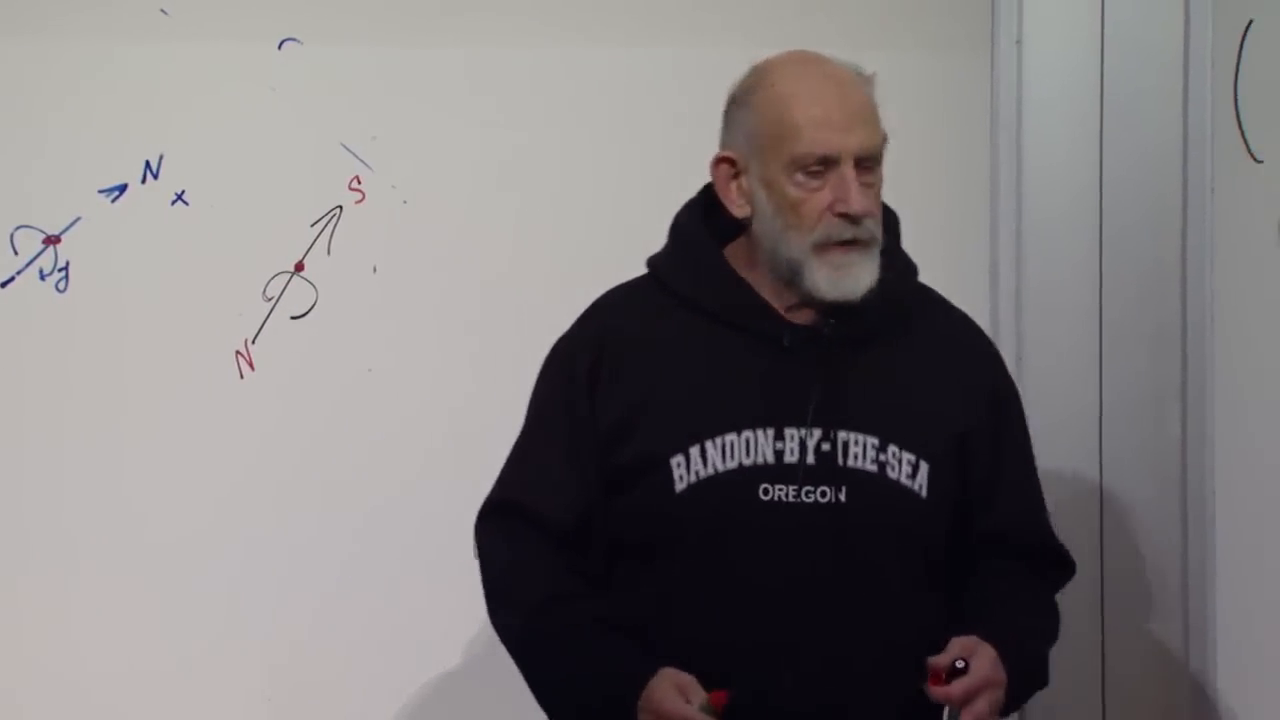
\includegraphics[width=0.94\linewidth]{lecture_08_frame_06.png}
\caption{时间反演论证中成对的磁轴与电荷位移草图。上方的紧凑 TikZ 图将变换内容从部分被擦除的现场板书中分离出来。}
\lectureframe{01:06:10}
\end{figure}

\begin{classroomqa}
\lecturetimestamp{01:06:38}
\audiencequestion{在时间反演下，电流和电荷都会反向吗？}
\lecturerresponse{电流反向是因为速度反向；电荷本身不反向。是电荷共轭 \(C\)，而不是时间反演 \(T\)，使电荷的符号反向。}
\end{classroomqa}

\begin{classroomqa}
\lecturetimestamp{01:07:01}
\audiencequestion{时间反演的反幺正性质是否意味着非相对论量子力学不具有时间反演不变性？}
\lecturerresponse{不是。反幺正性正是时间反演在量子力学中得到一致表示的方式：它对振幅取复共轭，并使动量和自旋反向。某个特定哈密顿量是否不变，是另一个问题。}
\end{classroomqa}

\begin{classroomqa}
\lecturetimestamp{01:07:19}
\audiencequestion{EDM 讨论是否要求电子具有有限体积，而不是点粒子？}
\lecturerresponse{不要求。点粒子的有效哈密顿量可以包含 \(-d_e\,\widehat{\mathbf S}\!\cdot\!\mathbf E\)。实验所问的是相反自旋取向是否获得不同的电场能量；它不必分辨字面意义上的延展电荷云。}
\end{classroomqa}

宇称不是弱相互作用的对称性；在弱相互作用的手征耦合中，它被最大程度地破坏。时间反演也不是严格的，但标准模型中已知的破坏只有极其微小的程度会进入电子 EDM。人们可以计算出非零的标准模型贡献，但它远低于这里所讨论的灵敏度。因此，零结果与标准模型一致，同时又能切入扩展---例如超对称及其他新相互作用---，这些扩展可以产生大得多的时间反演破坏。

基本实验思想很简单。磁场通过分裂自旋取向来揭示磁偶极矩。电场则会通过一个额外的与自旋相关的能量移动来揭示电偶极矩。真正的精密实验使用原子或分子、长的相干进动时间、外加场的反转以及对系统误差的仔细控制，而不是在朴素装置中孤立的电子。

\begin{classroomqa}
\lecturetimestamp{01:11:02}
\audiencequestion{电偶极矩搜寻是高能碰撞实验还是用实物对象做的实验？}
\lecturerresponse{它是精密桌面物理，使用束缚在受控原子或分子环境中的电子，并配合电场和磁场。它的能量很低，但它对微小破缺对称性的移动的灵敏度间接探测高能新物理。}
\end{classroomqa}

\begin{classroomqa}
\lecturetimestamp{01:12:21}
\audiencequestion{零结果是否约束了标准模型的哪些修改仍然可行？}
\lecturerresponse{原则上是的：每个模型都预言一个系数，因此占据某个参数区域。详细的数值排除需要专门计算，但一般逻辑是坚实的---与标准模型在更高精度上的一致，留给那些预言大电偶极矩的替代方案的空间就更少。}
\end{classroomqa}

\begin{classroomqa}
\lecturetimestamp{01:13:09}
\audiencequestion{量子信息守恒需要时间反演对称性吗？}
\lecturerresponse{不需要。即使哈密顿量在\(T\)下不变，幺正时间演化也守恒信息。固定磁场中的粒子是一个熟悉的例子：除非磁场也反转，否则磁场在时间反演的电影中选出一个取向，但量子演化仍然是幺正的。在局域洛伦兹不变量子场论的通常假设下，组合的\(CPT\)变换是一个对称性，但保证幺正性的并不是它。}
\end{classroomqa}

这一断裂现在可以结束了。零测量表明，在所述灵敏度下，电子没有探测到电偶极矩。它并没有说电子是一个球体，也没有推翻标准模型；它使一些被提出的偏离该模型的方案更难维持。

\section{回到二次量子化：傅里叶变换、动量模式与定域性}

我们当时在做二次量子化。让我们温和地重新开始，从普通单粒子波函数的一个熟悉事实出发，然后把它提升到算符。与傅里叶变换的联系是精确而简单的。

\subsection{从位置空间到动量空间}

小写\(\psi\)，而不是大写\(\Psi\)，是单粒子的波函数。在位置空间中，
\begin{equation}
P(x)=|\psi(x)|^2
\end{equation}
是在位置\(x\)找到粒子的概率密度。动量空间波函数是它的傅里叶变换，
\begin{equation}
\tilde{\psi}(p)=\int dx\,\psi(x)\,\frac{e^{-ipx}}{\sqrt{2\pi}},
\end{equation}
而逆关系是
\begin{equation}
\psi(x)=\int dp\,\tilde{\psi}(p)\,\frac{e^{ipx}}{\sqrt{2\pi}}.
\end{equation}
于是
\begin{equation}
P(p)=|\tilde{\psi}(p)|^2
\end{equation}
是动量\(p\)的概率密度。

我们使用\(\hbar=1\)。这两个变换互为逆变换：知道任一波函数就确定了另一个，而它们的绝对平方回答不同的测量问题。

对于自由粒子，
\begin{equation}
H=\frac{p^2}{2m},
\end{equation}
所以动量本征态也是能量本征态，它们在位置空间中的波函数是平面波，
\begin{equation}
\psi_p(x)\propto e^{ipx}.
\end{equation}
这就是二次量子化版本的出发点。

\begin{figure}[htbp]
\centering
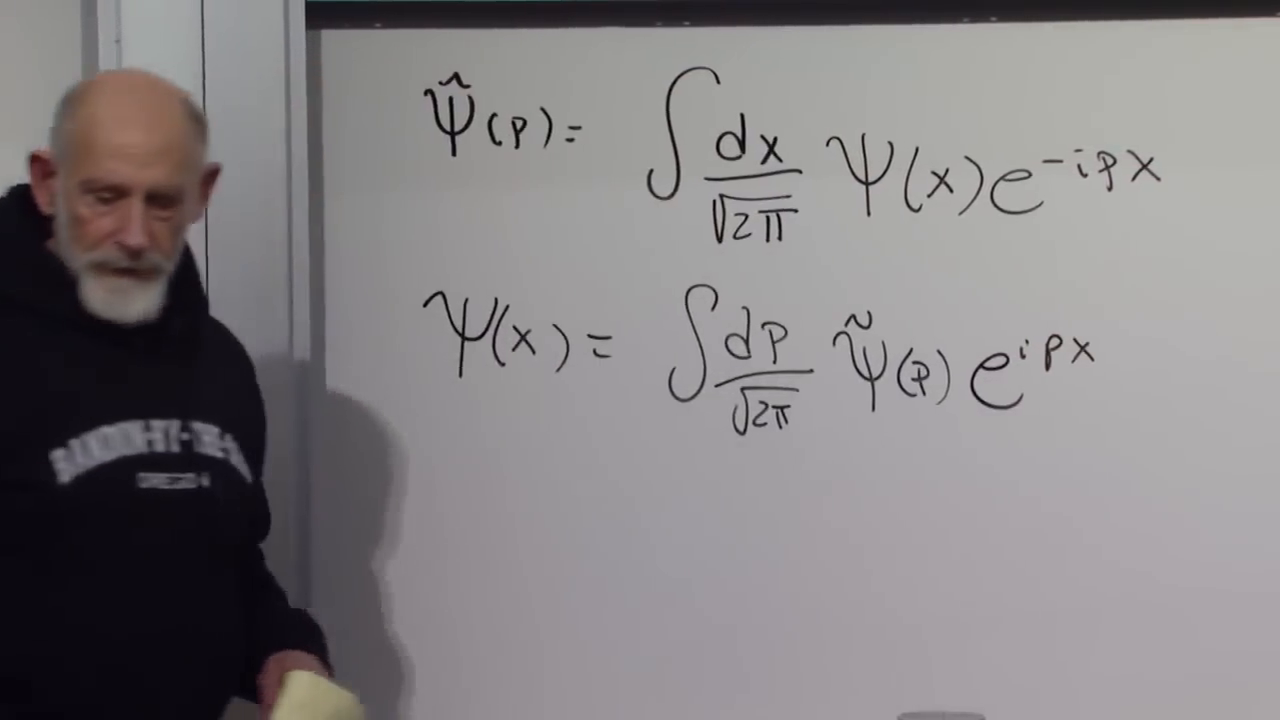
\includegraphics[width=0.94\linewidth]{lecture_08_frame_07.png}
\caption{单粒子波函数的位置--动量傅里叶对。小写\(\psi\)与接下来引入的大写场算符之间的区别是本质性的。}
\lectureframe{01:20:00}
\end{figure}

\subsection{位置空间和动量空间中的场算符}

现在回到场算符。在黑板上，它的湮灭和产生部分写作\(\Psi_-(x)\)和\(\Psi_+(x)\)。暂时保留这个记号，
\begin{align}
\Psi_-(x) &= \sum_i a_i\,\psi_i(x),\\
\Psi_+(x) &= \sum_i a_i^\dagger\,\psi_i^*(x).
\end{align}
这里\(\psi_i(x)\)是第\(i\)个模式的普通单粒子波函数，而\(a_i\)和\(a_i^\dagger\)在该模式中湮灭和产生粒子。从这一点起，方便地重新命名
\[
\Psi(x)\equiv \Psi_-(x),
\qquad
\Psi^\dagger(x)\equiv \Psi_+(x).
\]

对于自由粒子，离散模式标号\(i\)被连续动量标号\(p\)取代。使用平面波\(e^{ipx}\)，就得到标准的重构公式
\begin{align}
\Psi(x) &= \int \frac{dp}{\sqrt{2\pi}}\,a(p)\,e^{ipx},\\
\Psi^\dagger(x) &= \int \frac{dp}{\sqrt{2\pi}}\,a^\dagger(p)\,e^{-ipx}.
\end{align}
这些是普通傅里叶变换的场算符类比。它们可以像之前一样精确地求逆：
\begin{align}
a(p) &= \int \frac{dx}{\sqrt{2\pi}}\,\Psi(x)\,e^{-ipx},\\
a^\dagger(p) &= \int \frac{dx}{\sqrt{2\pi}}\,\Psi^\dagger(x)\,e^{ipx}.
\end{align}
\(1/\sqrt{2\pi}\)的因子是一种约定，选择它是为了使正变换和逆变换具有相同的归一化。

概念内容是直截了当的。\(\Psi^\dagger(x)\)在位置\(x\)处产生一个粒子，而\(a^\dagger(p)\)产生一个动量为\(p\)的粒子。位置空间和动量空间的产生算符互为傅里叶共轭，正如普通量子力学中\(\psi(x)\)和\(\tilde{\psi}(p)\)互为傅里叶共轭一样。

如果不存在动量为\(p\)的粒子，\(a(p)\)将态湮灭。如果存在该动量的粒子，它按通常的占据数系数移除一个。同样，\(\Psi(x)\)移除位置\(x\)处的一个粒子，这应在分布意义下理解，或在将其涂抹为波包之后理解。每种粒子都需要自己的场算符；一个场不能产生所有种类的粒子。

\subsection{玻色子对易子与分离测量的独立性}

下一个事实可以直接从定义推导出来。对于玻色子，
\begin{equation}
[a_i,a_j^\dagger]=\delta_{ij},
\qquad
[a_i,a_j]=0,
\qquad
[a_i^\dagger,a_j^\dagger]=0.
\end{equation}
连续版本为
\begin{equation}
[a(p),a^\dagger(p')]=\delta(p-p').
\end{equation}
现在从离散展开计算等时场对易子：
\begin{align}
[\Psi(x),\Psi^\dagger(y)]
&= \sum_{i,j}\psi_i(x)\psi_j^*(y)\,[a_i,a_j^\dagger] \\
&= \sum_i \psi_i(x)\psi_i^*(y) \\
&= \delta(x-y),
\end{align}
其中最后一步使用单粒子基的完备性。同样，
\begin{equation}
[\Psi(x),\Psi(y)]=0,
\qquad
[\Psi^\dagger(x),\Psi^\dagger(y)]=0.
\end{equation}

\begin{figure}[htbp]
\centering
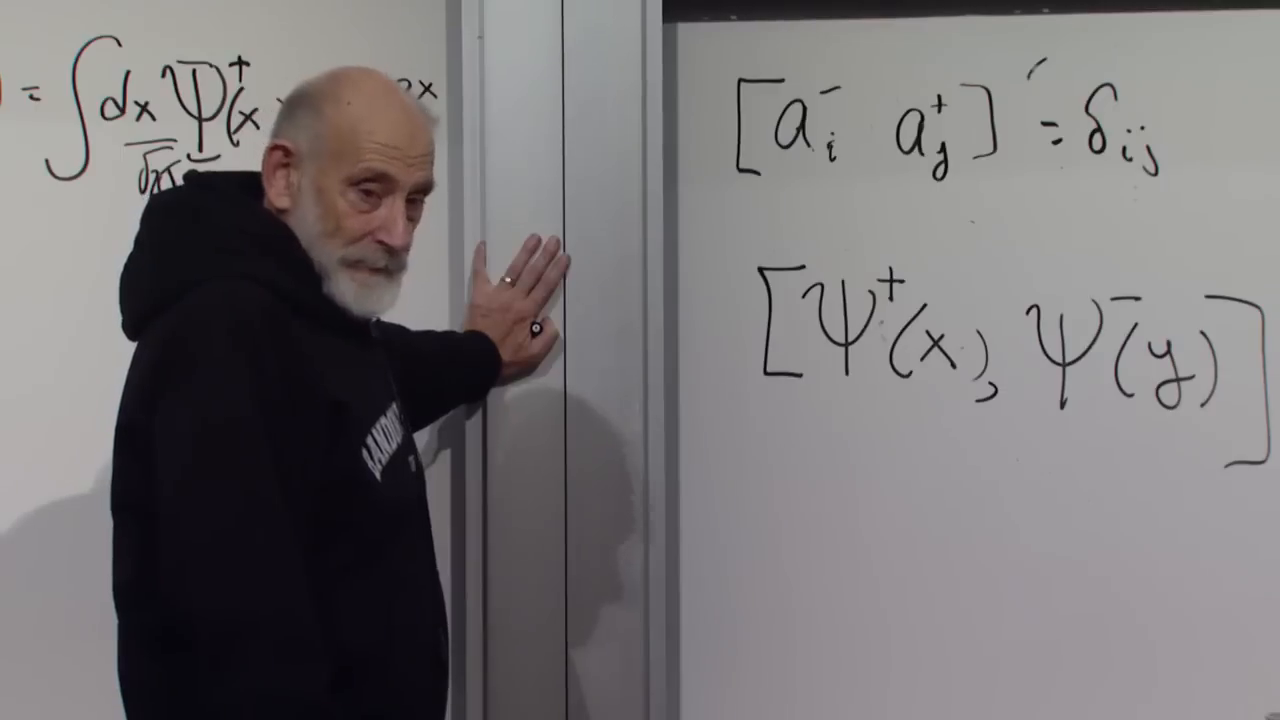
\includegraphics[width=0.94\linewidth]{lecture_08_frame_08.png}
\caption{黑板上的模式对易子及其位置空间对应物。完备性将\(\delta_{ij}\)变为空间{\proseunicodefont δ}分布\(\delta(x-y)\)。}
\lectureframe{01:31:00}
\end{figure}

重要之处不仅在于\(\Psi\)是非厄米的。定义厄米正交分量
\begin{equation}
Q(x)=\frac{\Psi(x)+\Psi^\dagger(x)}{\sqrt{2}},
\qquad
P(x)=\frac{\Psi(x)-\Psi^\dagger(x)}{i\sqrt{2}}.
\end{equation}
它们的同点对易子继承了{\proseunicodefont δ}分布。因此，这两个局域正交分量共轭，其意义与位置和动量共轭相同。试图使其中一个变尖锐会在另一个中产生不确定性。

\begin{classroomqa}
\lecturetimestamp{01:32:03}
\audiencequestion{当\(x=y\)时，{\proseunicodefont δ}函数意味着什么？对易子是否处处都很大？}
\lecturerresponse{{\proseunicodefont δ}是一个分布，而不是具有有限点值的普通函数。它在自变量分离时为零，只有在与检验函数积分后才给出有限结果。将场涂抹到有限探测器区域上，会把形式上的同点奇异性变为两个模式之间通常的有限正则对易子。}
\end{classroomqa}

然而，对于\(x\neq y\)，等时对易子为零。局域在两个不相交区域中的操作可以独立进行：测量这里的场不会给那里的场一个量子踢动。这是相对论微观因果性的非相对论等时前身。在相对论理论中，物理局域可观测量在类空间隔处对易，因为在那里没有光信号能连接两个事件。

与非对易可观测量的对比是熟悉的。由于\([x,p]=i\)，精确的位置测量会扰动动量，而精确的动量态会在位置上扩展。由于不同自旋分量不对易，将其中一个分量制备得很尖锐会使另一个不确定。分离的局域可观测量之间若对易子非零，类似地意味着一个区域中的操作会扰动另一个区域，这与所要求的因果独立性相矛盾。

\begin{classroomqa}
\lecturetimestamp{01:37:51}
\audiencequestion{EPR和纠缠实验是否表明这里的测量对远处的测量有影响？}
\lecturerresponse{它们表明的是关联，而不是可控的因果影响。纠缠结果违反经典因子化，但远处探测器处的局域统计不能通过选择或执行这里的测量来改变。类空分离可观测量的对易性，就是这种无信号独立性背后的算符陈述。}
\end{classroomqa}

下一次代数会改变。费米子产生和湮灭算符满足反对易关系。若天真地看待，分离点处的费米子场不对易，因此场本身不能被解释为可直接测量的玻色型可观测量。物理的费米型可观测量是偶组合---密度、流、应力张量---，而这些局域可观测量恢复了所需的类空对易性。这就是进入费米子版本二次量子化的入口。
